\chapter{Gap Reconstruction}
One of the more common problems in citizen science projects is gaps in data. This can happen either if the network connection is unstable or the test equipment gets prematurely turn off. This can greatly degrade the data quality, and lead to errors in the application. One way to deal with this problem is do use mathematical gap filling techniques to come with a qualified guess on how the data would look like in the gap. 

In order to use this methods we must assume that the missing data in the gap follows the same behaviour as the data on each side off the gap. Is the signal so stochastic that this is not the case gap filling is not recommended\citep{RefWorks:10}. 

In the case of the SmartHG project the data can be seen to have a part that is dependency on the previous and future data plus a stochastic part that are determined by the user and the appliance. Due to the stochastic part a perfect reconstruction is not possible, but it is the hypotheses that the non stochastic part is still so dominant that a decent reconstruction is possible. 
\section{Gaps In SmartHG Dataset}
The gaps in the SmartHG project dataset is caused by a lot of different sources. This makes the type of gaps different from case to case. Three aspects of a gap is important for the gap filling: The size of the gap, the data known before the gap, and the data known after the gap. 
\subsection{Gap Size}
Looking at the different gaps in the dataset we see that the normal gap is relatively small. This can be seen on figure \ref{fig:GapSize}
\begin{figure}[H]
\centering
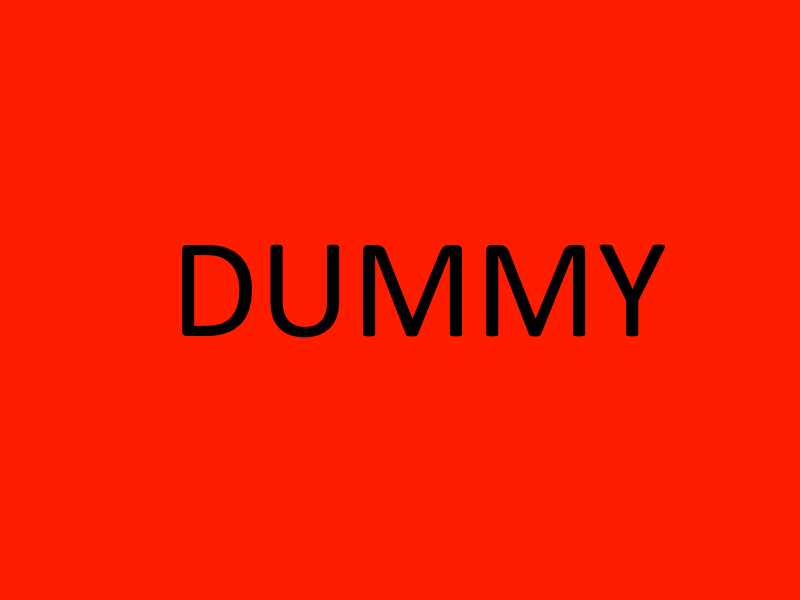
\includegraphics[width=0.3\textwidth]{billeder/DUMMY.png}
\caption{Gap size}
\label{fig:GapSize}
\end{figure}
This is good since the signal part stochastic. The grater the gap, the greater influence does the stochastic part have on the signal. Smaller gaps can therefore be fixed with greater success. 
\subsection{Past And Future Availability}
It is also important how many samples are available on the left and right side of the gap. If there is a lot of gaps in the signal it can create a scenario where there only is a small amount of good data between the gaps. This makes it hard to reconstruct the data, since there is very few points to extract information about the region. 
\begin{figure}[H]
\centering
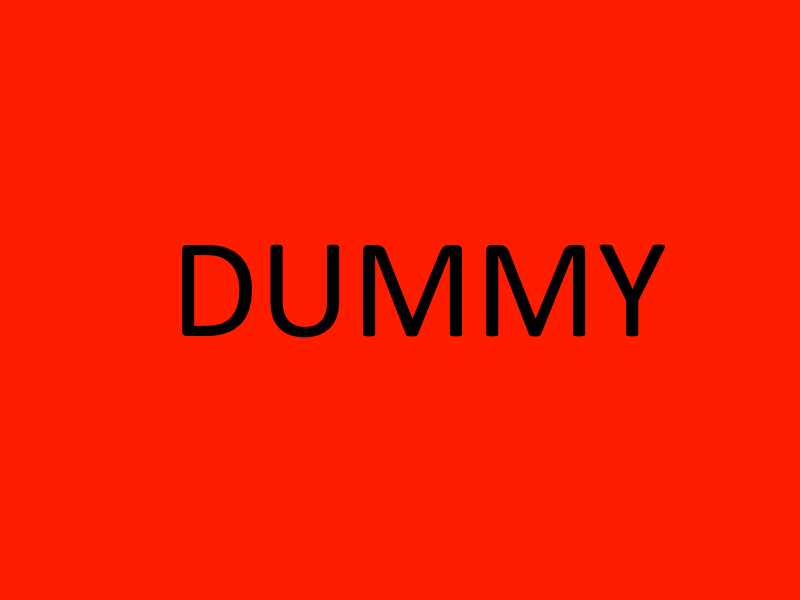
\includegraphics[width=0.3\textwidth]{billeder/DUMMY.png}
\caption{Past and future availability}
\label{fig:PAF}
\end{figure}
As seen on figure \ref{fig:PAF} \fxnote{Write something more when you know the result}

\section{Gap Filling Methods}
Various methods exists for gap filling. Five popular algorithms have been implemented and validated on the SmartHG project data.

\subsection{Papoulis-Gerchberg Algorithm}
\lipsum[7] %dummy text 
\subsection{Wiener Filling Algorithm}
\lipsum[7] %dummy text 
\subsection{Spatio-Temporal Filling Algorithm}
\lipsum[7] %dummy text 
\subsection{Envelope Filling Algorithm}
\lipsum[7] %dummy text 
\subsection{Empirical Mode Decomposition Filling Algorithm}
\lipsum[7] %dummy text 

\section{SmartHG Dataset Reconstruction}

\section{Related Work}